\documentclass[12pt]{article}

\usepackage[margin = .8in]{geometry}
\usepackage{amsmath}
\usepackage{graphicx}
\usepackage{multicol, enumerate}

\usepackage{fancyhdr}
\pagestyle{fancy}

\lhead{Math F113X: Numbers and Society}
\rhead{Date: \hspace{1in}}

\usepackage{tikz}
\usetikzlibrary{calc,trees,positioning,arrows,fit,shapes,calc}
\usetikzlibrary{patterns}
\usepackage{pgfplots}

\usepackage{longtable}
\usepackage{tabularx}

\newcommand{\ds}{\displaystyle}
\newcommand{\ans}[1][1in]{\rule{#1}{.5pt}}

\newcommand{\points}[1]{(#1 points.)}		% Trying to be lazy.

\usepackage{array}
\newcolumntype{L}[1]{>{\raggedright\let\newline\\\arraybackslash\hspace{0pt}}m{#1}}
\newcolumntype{C}[1]{>{\centering\let\newline\\\arraybackslash\hspace{0pt}}m{#1}}
\newcolumntype{R}[1]{>{\raggedleft\let\newline\\\arraybackslash\hspace{0pt}}m{#1}}
\newcommand{\red}[1]{\textcolor{red}{#1}}

%\topmargin -1in
%\textheight 9.5in
%\oddsidemargin -0.3in
%\evensidemargin \oddsidemargin
%\pagestyle{empty}
%%\marginparwidth 0.5in
%\textwidth 7in
%\parindent 0in

%--------------------------------------------------------------------------------------------------------------------------------------------------------------------------
%						Document
%--------------------------------------------------------------------------------------------------------------------------------------------------------------------------


\begin{document}
%\pagestyle{fancy}
\begin{center}
{\Large  Worksheet 7 (Fair Division 2): The Lone Divider Method	}
\end{center}



\noindent \textbf{Group Names:} \hrulefill \\
%-------------------------------------------------------------------------------------------------------------
%						Assignment
%-----------------------------------------------------------------------------------------------------


%\begin{minipage}[b]{.6\linewidth}
Tom, Fred, and Janet are dividing a super-fancy gourmet cake worth \$36 that is equal parts strawberry, vanilla and chocolate.% Tom likes vanilla and strawberry the same but does not like chocolate at all. Fred will eat vanilla but likes strawberry twice as much as vanilla and likes chocolate three times as much as vanilla.

%\end{minipage}

\begin{center}
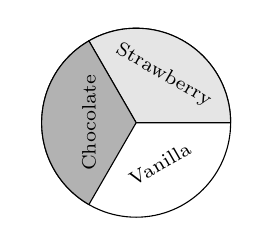
\begin{tikzpicture}
\def\r{1.2}
\draw (0,0) circle (\r cm);
\filldraw[fill= gray!20 ] (0,0) -- (0:\r) arc (0:120:\r) -- (0,0);
\path (60:.7) node[rotate = -30]{{{\scriptsize Strawberry}}};
%\path node[right] (240:1) {{\scriptsize Strawberry}};
\filldraw[fill = gray!60 ] (0,0) -- (120:\r) arc (120:240:\r) -- (0,0);
\path (120+60:\r/2) node[rotate = 90]{{{\scriptsize Chocolate}}};
\path (-60:\r/2) node[rotate = 30]{{{\scriptsize Vanilla}}};
\end{tikzpicture}
\end{center}

%
%\begin{minipage}[b]{.4\linewidth}

%\end{minipage}

\begin{enumerate}
\item How much value is a fair share of the cake? \ans

\item Tom divides the cake into three portions (not necessarily according to flavors!) that he values equally. Janet and Fred value the portions according to the following table:

\begin{center}
\begin{tabular}{| c | c | c | c |}
\hline
& portion 1& portion 2 & portion 3\\ \hline \hline
Tom & \$12 & \$12 & \$12 \\ \hline
Janet & \$7 & \$18 & \$11 \\ \hline
Fred & \$15 & \$18 & \$3\\ \hline
\end{tabular}
\end{center}

\begin{enumerate}
\item Which portion(s) represent a fair share  for Janet? \ans[2in]
\item Which portion(s) represent a fair share  for Fred? \ans[2in]
\item Is it possible to distribute the portions of cake to the three people so that everyone gets a portion that is a fair share for them? If so, explain how to do so; if not, explain what happens next.

\vfill
\end{enumerate}

\item It turns out that Janet and Fred changed their mind on how they value the portions of cake that Tom gave. Their new values are given in the following table:
\begin{center}
\begin{tabular}{| c | c | c | c |}
\hline
& portion 1& portion 2 & portion 3\\ \hline \hline
Tom & \$12 & \$12 & \$12 \\ \hline
Janet & \$6 & \$20 & \$10 \\ \hline
Fred & \$7 & \$18 & \$11 \\ \hline
\end{tabular}
\end{center}

\begin{enumerate}
\item Which portion(s) represent a fair share  for Janet? \ans[2in]
\item Which portion(s) represent a fair share  for Fred? \ans[2in]
\item Is it possible to distribute the portions of cake to the three people so that everyone gets a piece that is a fair share for them? If so, explain how to do so; if not, explain what happens next.

\vfill

\end{enumerate}


\newpage

\item In a final cake scenario, suppose that Tom was the lone divider, and the people valued the cake as follows:

\begin{itemize}
\item Tom likes all three flavors equally.
\item Janet likes strawberry twice as much as vanilla. She likes chocolate SIX times as much as vanilla.
\item Fred's values are listed in the table.
\end{itemize}

\begin{enumerate}

\item If Tom portioned the cake into three pieces where each piece was a single flavor, determine the valuations that Janet would assign to the pieces of cake (fill in the table).

\bigskip

%\begin{center}
{  % Start local group
\renewcommand{\arraystretch}{1.4} 
\begin{tabular}{| c | c | c | c |}
\hline
& vanilla& chocolate  & strawberry \\ \hline \hline
Tom & \$12 & \$12 & \$12 \\ \hline
Janet&  &  &  \\ \hline
Fred& \$11& \$15 & \$10  \\
\hline
\end{tabular}
}
%\end{center}
\bigskip

\item Which pieces represent a fair share  for Janet? \ans[2in]
\item Which pieces represent a fair share  for Fred? \ans[2in]
\item Explain why it is not possible to distribute Tom's pieces of cake so that everyone gets a fair share.

\vfill

\item Choose a piece of cake to assign to Tom, and explain why you chose that piece.

\vfill

\item Now, use Divider-Chooser to determine the division of the rest of the cake. Suppose that you flipped a coin, and Janet was chosen to be the divider. 

\begin{enumerate}
\item Label Janet's values on the cake and draw a partition of the cake on Janet's side that Janet might make as the divider. (Don't forget to exclude the part Tom already has!)
\item Label Fred's values and determine the value of Janet's cake division to him.
\item What pieces do Janet and Fred end up with after divider-chooser?
\end{enumerate}

\bigskip

\begin{center}
\def\r{1.2}
\begin{tikzpicture}
\path (90:\r) node[above] {Janet's Values};
\draw (0,0) circle (\r cm);
\filldraw[fill= gray!20 ] (0,0) -- (0:\r) arc (0:120:\r) -- (0,0);
\filldraw[fill = gray!60 ] (0,0) -- (120:\r) arc (120:240:\r) -- (0,0);
\end{tikzpicture}
\hspace{1cm}
\begin{tikzpicture}
\path (90:\r) node[above] {Fred's Values};
\draw (0,0) circle (\r cm);
\filldraw[fill= gray!20 ] (0,0) -- (0:\r) arc (0:120:\r) -- (0,0);
\filldraw[fill = gray!60 ] (0,0) -- (120:\r) arc (120:240:\r) -- (0,0);
\end{tikzpicture}
\end{center}

\end{enumerate}

\vfill




%\item Challenge: Suppose that another friend, Janet, likes vanilla 3 times as much as she likes strawberry and chocolate, which she likes equally. How much does she value each of the three pieces?
%
%%\vspace{1.5in}
%\hfill\begin{tikzpicture}
%\draw (0,0) circle (\r cm);
%\filldraw[fill= gray!20 ] (0,0) -- (0:\r) arc (0:120:\r) -- (0,0);
%\filldraw[fill = gray!60 ] (0,0) -- (120:\r) arc (120:240:\r) -- (0,0);
%\path (90:\r) node [above] {Janet's Values};
%\end{tikzpicture}
%
%Strawberry \ans Vanilla \ans Chocolate \ans
%
\end{enumerate}

\end{document}

%-------------------------------------------------------------------------------------------------------------------------------------------------------------------------------------------------------------------

%%% Local Variables:
%%% mode: latex
%%% TeX-master: t
%%% End:
